% !TEX root = main.tex
\documentclass[a4paper, UKenglish, 11pt]{uiomaster}
\usepackage{lipsum}
\usepackage[subpreambles=true]{standalone}
\usepackage[table,xcdraw]{xcolor}
\documentclass[border=3pt,tikz]{standalone}
\usepackage{amsmath} % for aligned
%\usepackage{amssymb} % for \mathbb
\usepackage{tikz}
%\usepackage{etoolbox} % for \ifthen
\usepackage{listofitems} % for \readlist to create arrays
\usetikzlibrary{arrows.meta} % for arrow size
\usepackage[outline]{contour} % glow around text
\contourlength{1.4pt}

\tikzset{>=latex} % for LaTeX arrow head
\usepackage{xcolor}
\colorlet{myred}{red!80!black}
\colorlet{myblue}{blue!80!black}
\colorlet{mygreen}{green!60!black}
\colorlet{myorange}{orange!70!red!60!black}
\colorlet{mydarkred}{red!30!black}
\colorlet{mydarkblue}{blue!40!black}
\colorlet{mydarkgreen}{green!30!black}
\tikzstyle{node}=[thick,circle,draw=myblue,minimum size=22,inner sep=0.5,outer sep=0.6]
\tikzstyle{node in}=[node,green!20!black,draw=mygreen!30!black,fill=mygreen!25]
\tikzstyle{node hidden}=[node,blue!20!black,draw=myblue!30!black,fill=myblue!20]
\tikzstyle{node convol}=[node,orange!20!black,draw=myorange!30!black,fill=myorange!20]
\tikzstyle{node out}=[node,red!20!black,draw=myred!30!black,fill=myred!20]
\tikzstyle{connect}=[thick,mydarkblue] %,line cap=round
\tikzstyle{connect arrow}=[-{Latex[length=4,width=3.5]},thick,mydarkblue,shorten <=0.5,shorten >=1]
\tikzset{ % node styles, numbered for easy mapping with \nstyle
  node 1/.style={node in},
  node 2/.style={node hidden},
  node 3/.style={node out},
}
\def\nstyle{int(\lay<\Nnodlen?min(2,\lay):3)} % map layer number onto 1, 2, or 3

\begin{document}

\section{Localizing Single Dipole Sources and Amplitudes}

In the next problem, we introduce the concept of various amplitudes for single current dipole sources, which adds an additional dimension to our network's output. Besides predicting the coordinates of the dipoles for each sample, the network now also estimates the magnitude of the dipole signals. In real-world scenarios, it might be of interest to not only pinpoint the source of the abnormal activity but also comprehend the extent of abnormality. By incorporating amplitude prediction into our network, we gain valuable insights into the problem at hand and achieve a deeper understanding of the underlying brain activity.

We start off by introducing the extensions of out DiLoc network, that now consists of 8 hidden layers. Whereas the DiLoc neural network introduced for the purpose of localizing single current dipoles had an decreasing architecture with an increasing number of layers, the new DiLoc network know has a slightly more complicated structure.

% NEURAL NETWORK with coefficients, shifted
\begin{tikzpicture}[x=2.2cm,y=1.4cm]
  \message{^^JNeural network, shifted}
  \readlist\Nnod{8,10,16,8,7,6,5,5,4} % array of number of nodes per layer
  \readlist\Nstr{231,512,1024,512,256,128,64,32,4} % array of string number of nodes per layer
  \readlist\Cstr{\strut x,a^{(\prev)},a^{(\prev)},a^{(\prev)},y} % array of coefficient symbol per layer
  \def\yshift{0.5} % shift last node for dots

  \message{^^J  Layer}
  \foreachitem \N \in \Nnod{ % loop over layers
    \def\lay{\Ncnt} % alias of index of current layer
    \pgfmathsetmacro\prev{int(\Ncnt-1)} % number of previous layer
    \message{\lay,}
    \foreach \i [evaluate={\c=int(\i==\N); \y=\N/2-\i-\c*\yshift;
                 \index=(\i<\N?int(\i):"\Nstr[\lay]");
                 \x=\lay; \n=\nstyle;}] in {1,...,\N}{ % loop over nodes
      % NODES
      \node[node \n] (N\lay-\i) at (\x,\y) {$\Cstr[\lay]_{\index}$};

      % CONNECTIONS
      \ifnum\lay>1 % connect to previous layer
        \foreach \j in {1,...,\Nnod[\prev]}{ % loop over nodes in previous layer
          \draw[connect,white,line width=1.2] (N\prev-\j) -- (N\lay-\i);
          \draw[connect] (N\prev-\j) -- (N\lay-\i);
          %\draw[connect] (N\prev-\j.0) -- (N\lay-\i.180); % connect to left
        }
      \fi % else: nothing to connect first layer

    }
    \path (N\lay-\N) --++ (0,1+\yshift) node[midway,scale=1.5] {$\vdots$};
  }

  % LABELS
  \node[above=5,align=center,mygreen!60!black] at (N1-1.90) {input\\[-0.2em]layer};
  \node[above=2,align=center,myblue!60!black] at (N3-1.90) {hidden layers};
  \node[above=10,align=center,myred!60!black] at (N\Nnodlen-1.90) {output\\[-0.2em]layer};

\end{tikzpicture}


We assign amplitudes to each dipole ranging between 1 and 10 nA$\mu$m. Although the dataset still has the same number of features, the number of target values increases by 1. Figure \ref{fig:dipole_w_amplitude_example} provides two examples from the dataset, where the dipole location remains constant while the amplitude of the dipole signal varies. In such cases, the shape of the EEG signal will remain consistent, but the magnitude of the EEG signal will be highest for the dipole with the largest amplitude.

\begin{figure}[!htb]
    \centering
    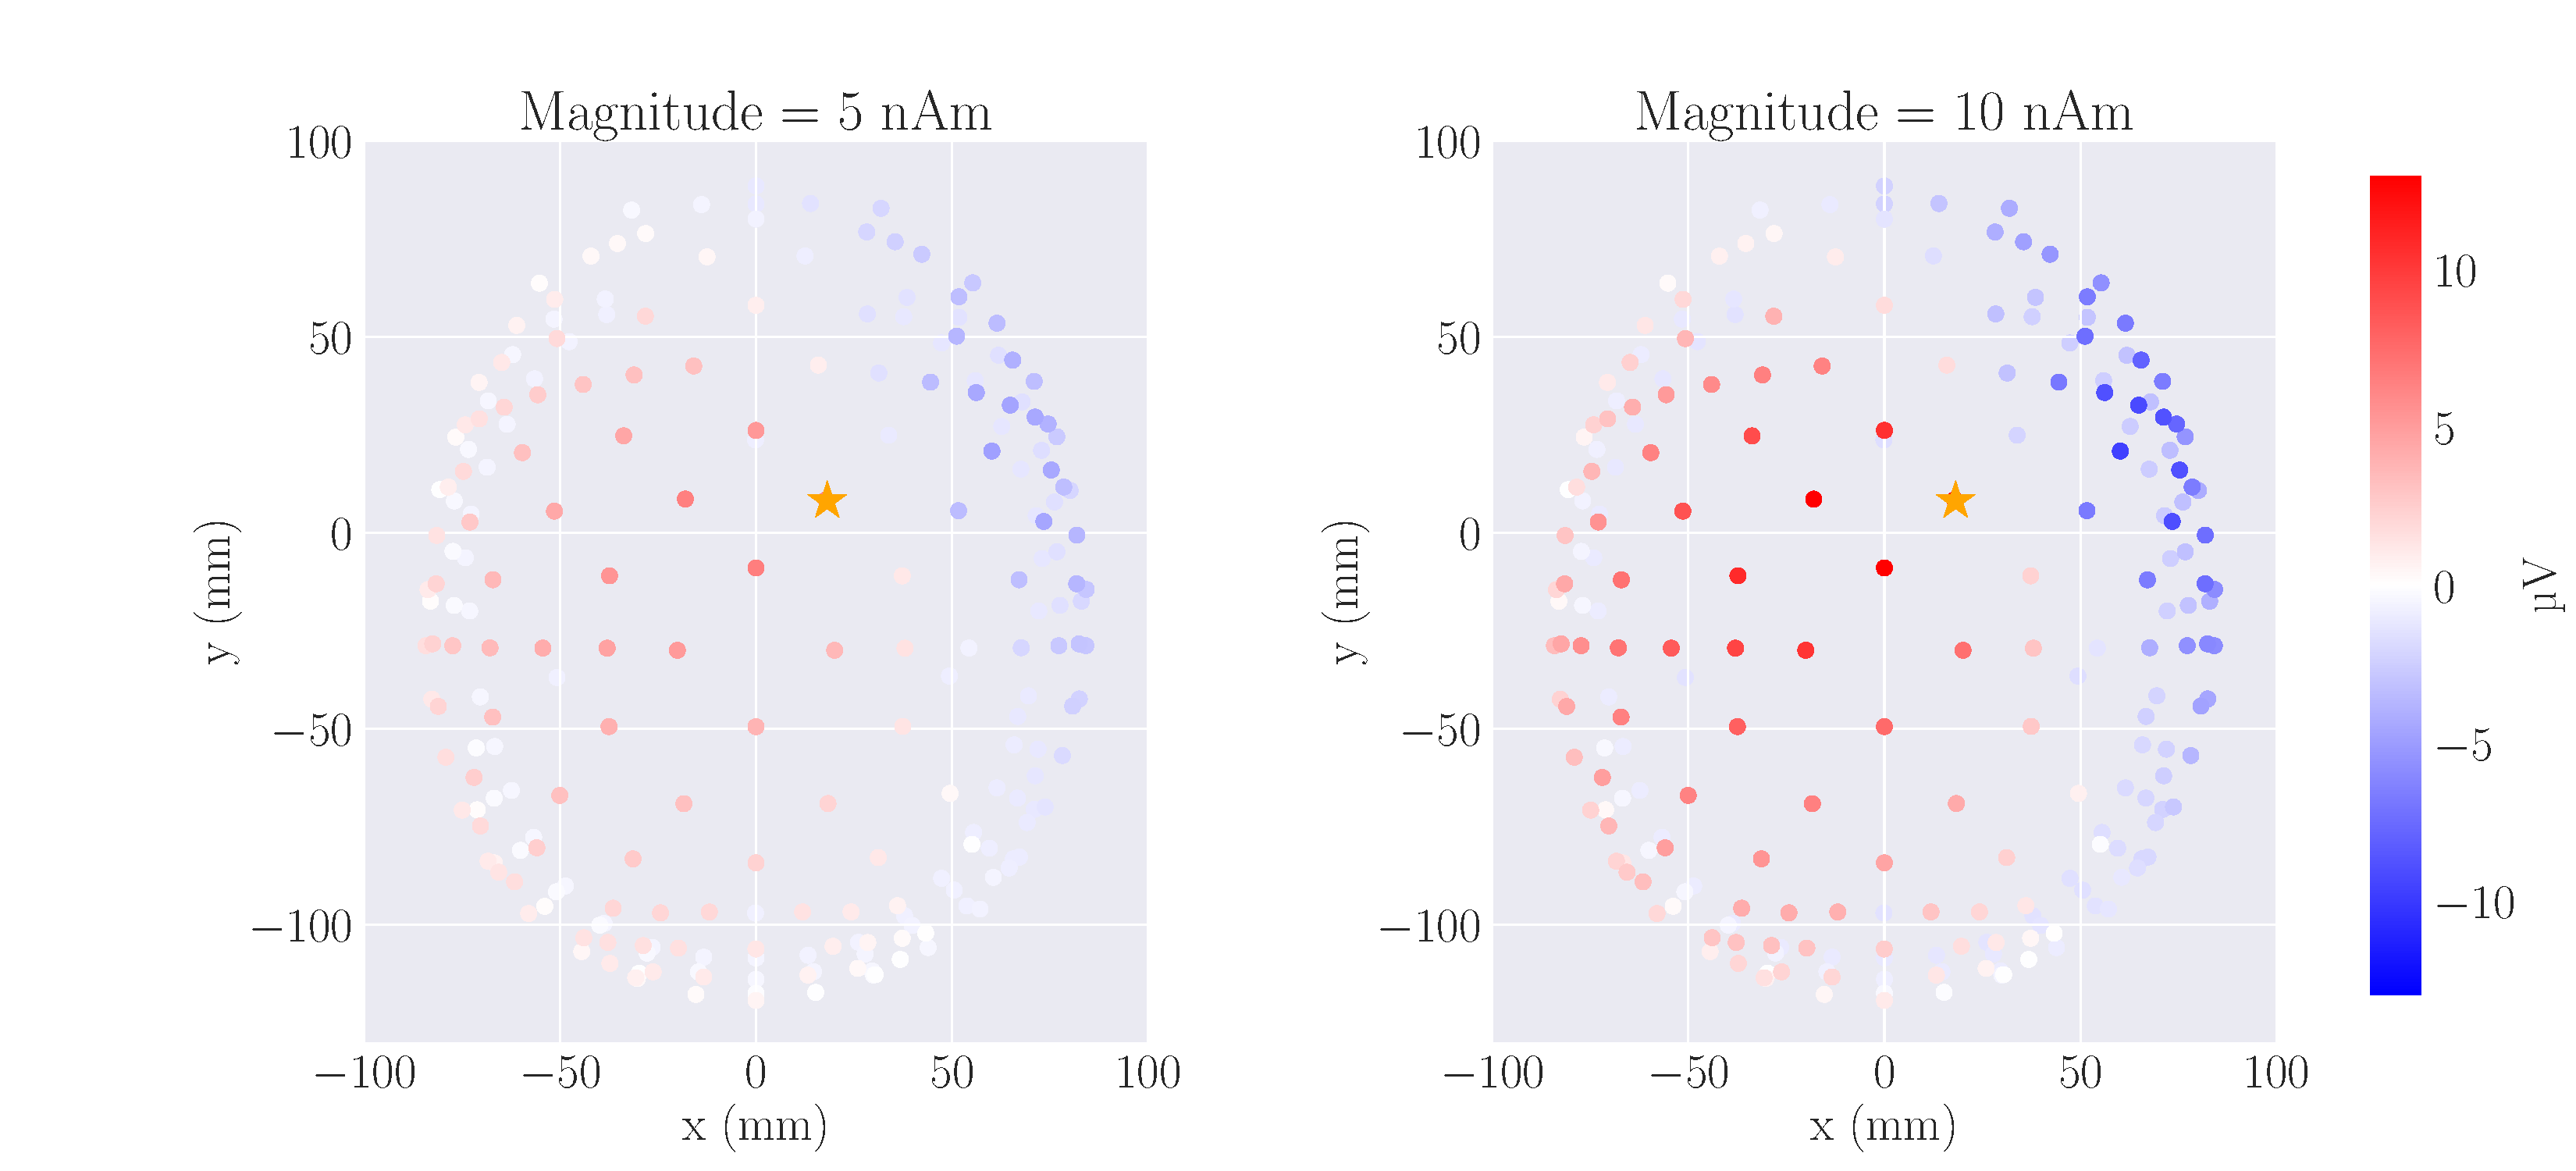
\includegraphics[width=\linewidth]{figures/dipole_w_amplitude_example.pdf}
    \caption{EEG data for two samples with current dipole amplitude equal to 5 and 10.}
    \label{fig:dipole_w_amplitude_example}
\end{figure}

To evaluate the network's performance, we track the accuracy as a function of training epochs, as shown in Figure \ref{fig:dipole_w_amplitude_example_accuracy}. The plot demonstrates a clear trend of decreasing loss with an increasing number of epochs, indicating that the network effectively captures the underlying patterns in the data. Furthermore, both the training and validation loss stabilize after approximately 400 epochs, suggesting that the network has reached a relatively optimal performance level.

\begin{figure}[!htb]
    \centering
    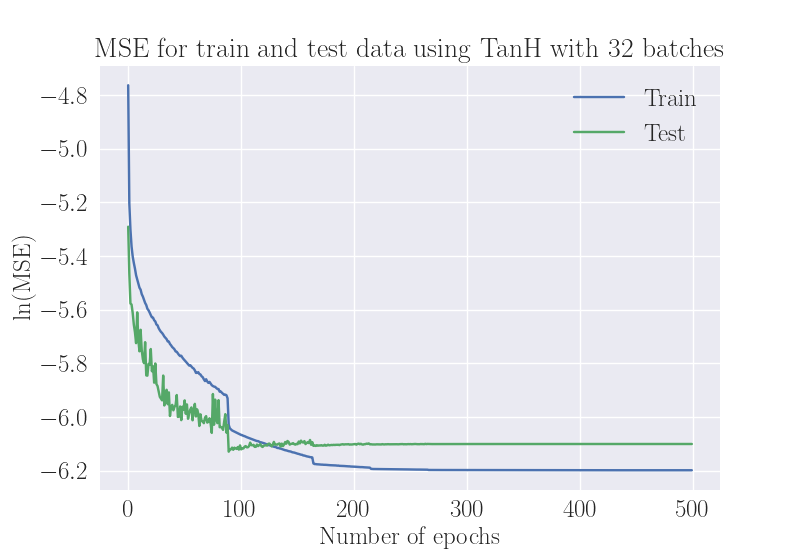
\includegraphics[width=\linewidth]{figures/MSE_TEST_dipole_w_amplitude_500_SGD_lr0.9_wd1e-05_bs32_TanH_32_500_N_dipoles_1.png}
    \caption{EEG data for two samples with current dipole amplitude equal to 5 and 10.}
    \label{fig:dipole_w_amplitude_example_accuracy}
\end{figure}



\section{Region of Active Correlated Current Dipoles}

Some results for the prediction of the size and location of current dipole populations.

\begin{figure}[!htb]
    \centering
    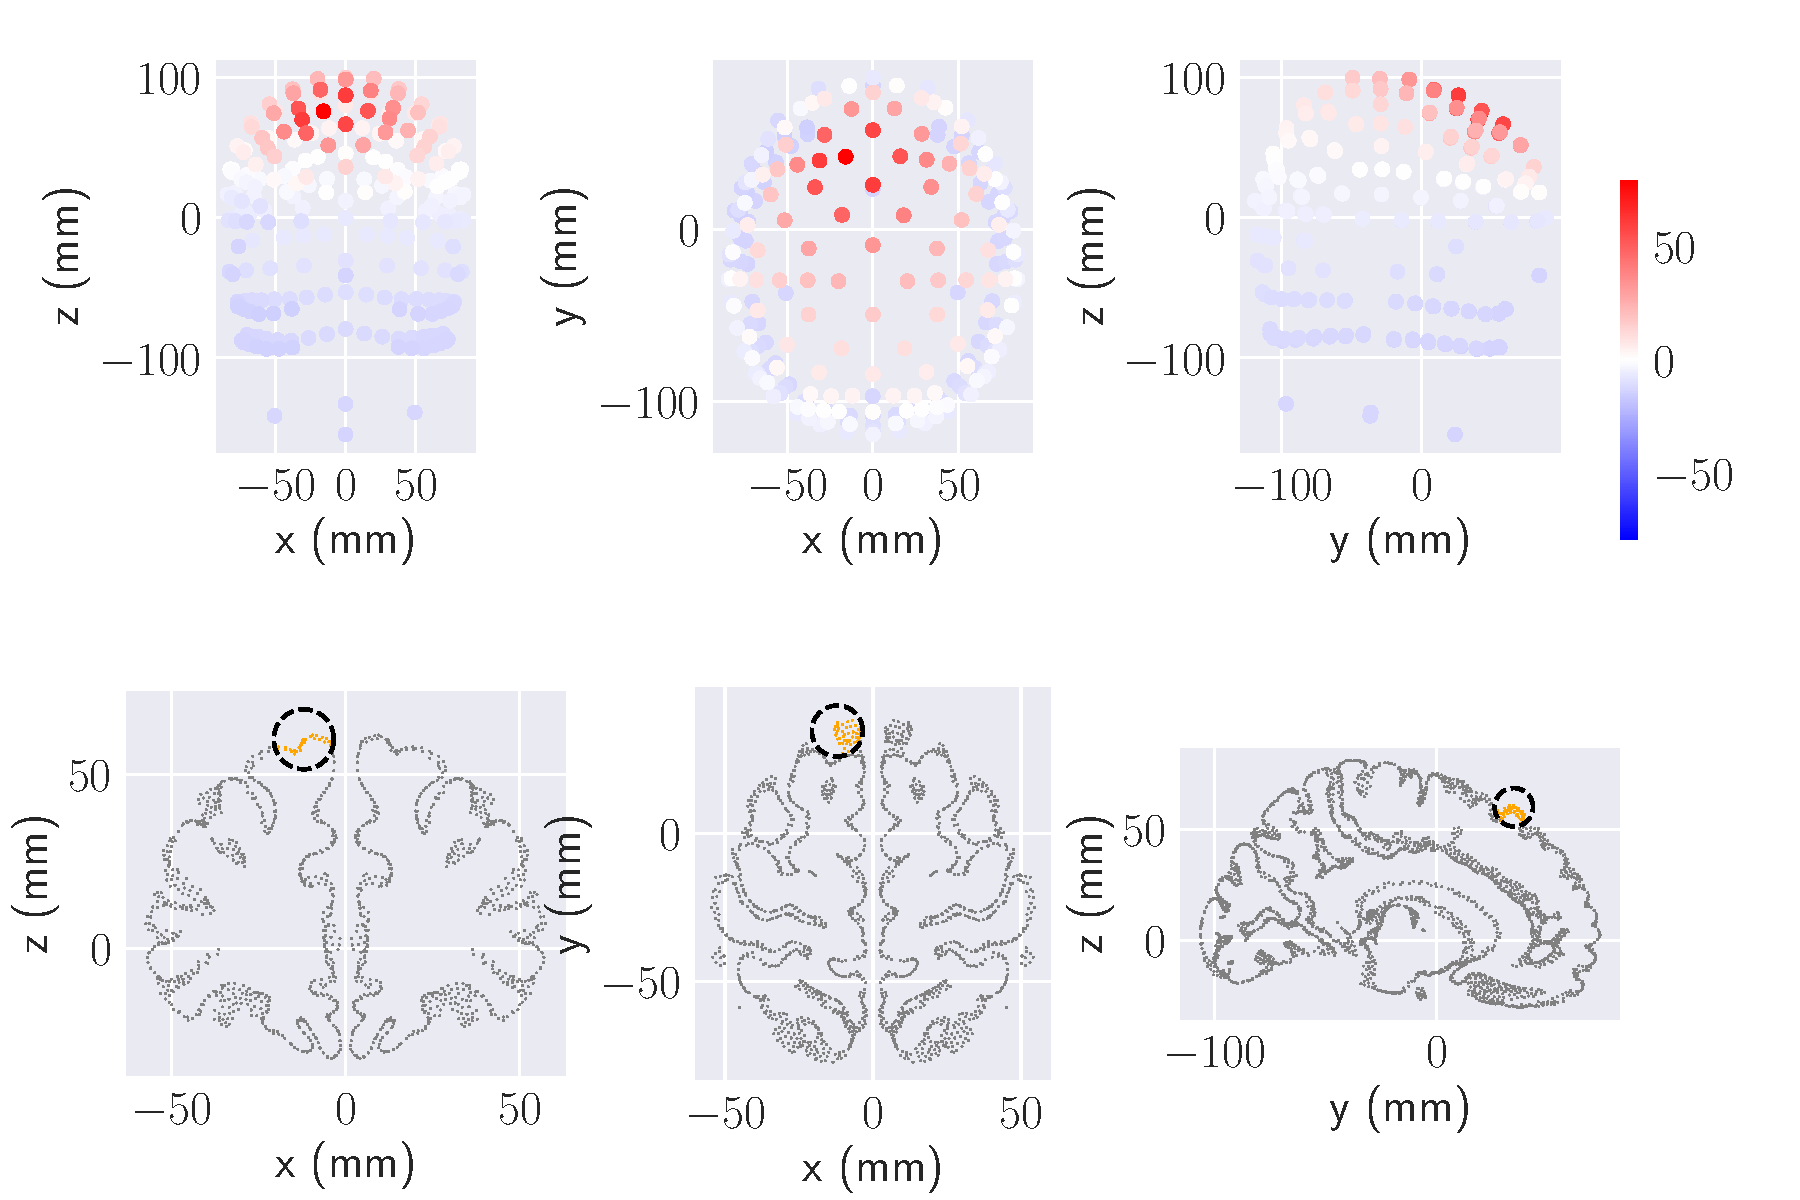
\includegraphics[width=\linewidth]{../Code/plots/finals/new_dipole_area_reduced_0.pdf}
    \caption{EEG for a sample containing a spherical population of current dipole sources with a random center within the celebral cortex. The EEG measure is seen from both sides (x-, z-plane and y-, z-plane) and above (the x-, y-plane). EEG electrode locations are presented as filled circels, where the color of the fill represents the amplitude of the measured signal for the given electrode.}
    \label{fig:dipole_area}
\end{figure}

\begin{figure}[!htb]
    \centering
    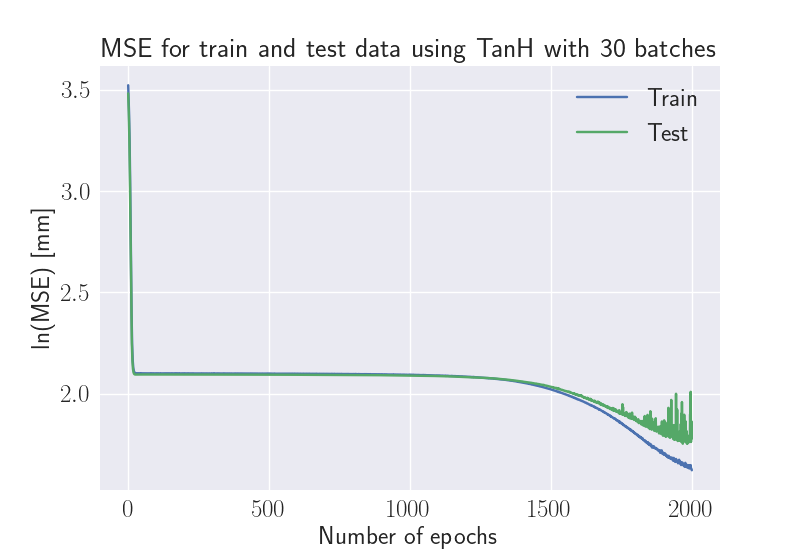
\includegraphics[width=\linewidth]{../Code/plots/finals/normalized_dipole_area.png}
    \caption{The validation accuracy for the simple Feed Forward Neural Network, predicting both center and radius for 10 000 samples, for 2000 epochs, with a learning rate equal to 0.0001.}
    \label{fig:dipole_area_result}
\end{figure}

\begin{figure}[!htb]
    \centering
    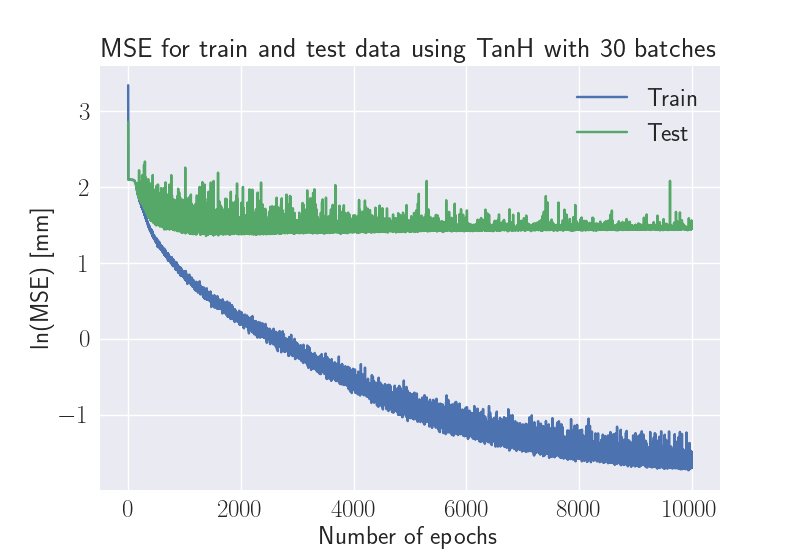
\includegraphics[width=\linewidth]{../Code/plots/finals/MSE_dipole_area_lr0.001_l1_20mm_TanH_30_10000.png}
    \caption{The validation accuracy for the simple Feed Forward Neural Network, predicting both center and radius for 10 000 samples, for 10000 epochs, with a learning rate equal to 0.001.}
    \label{fig:dipole_area_result}
\end{figure}





\section{Localizing Multiple Dipole Sources}
\begin{figure}[!htb]
    \centering
    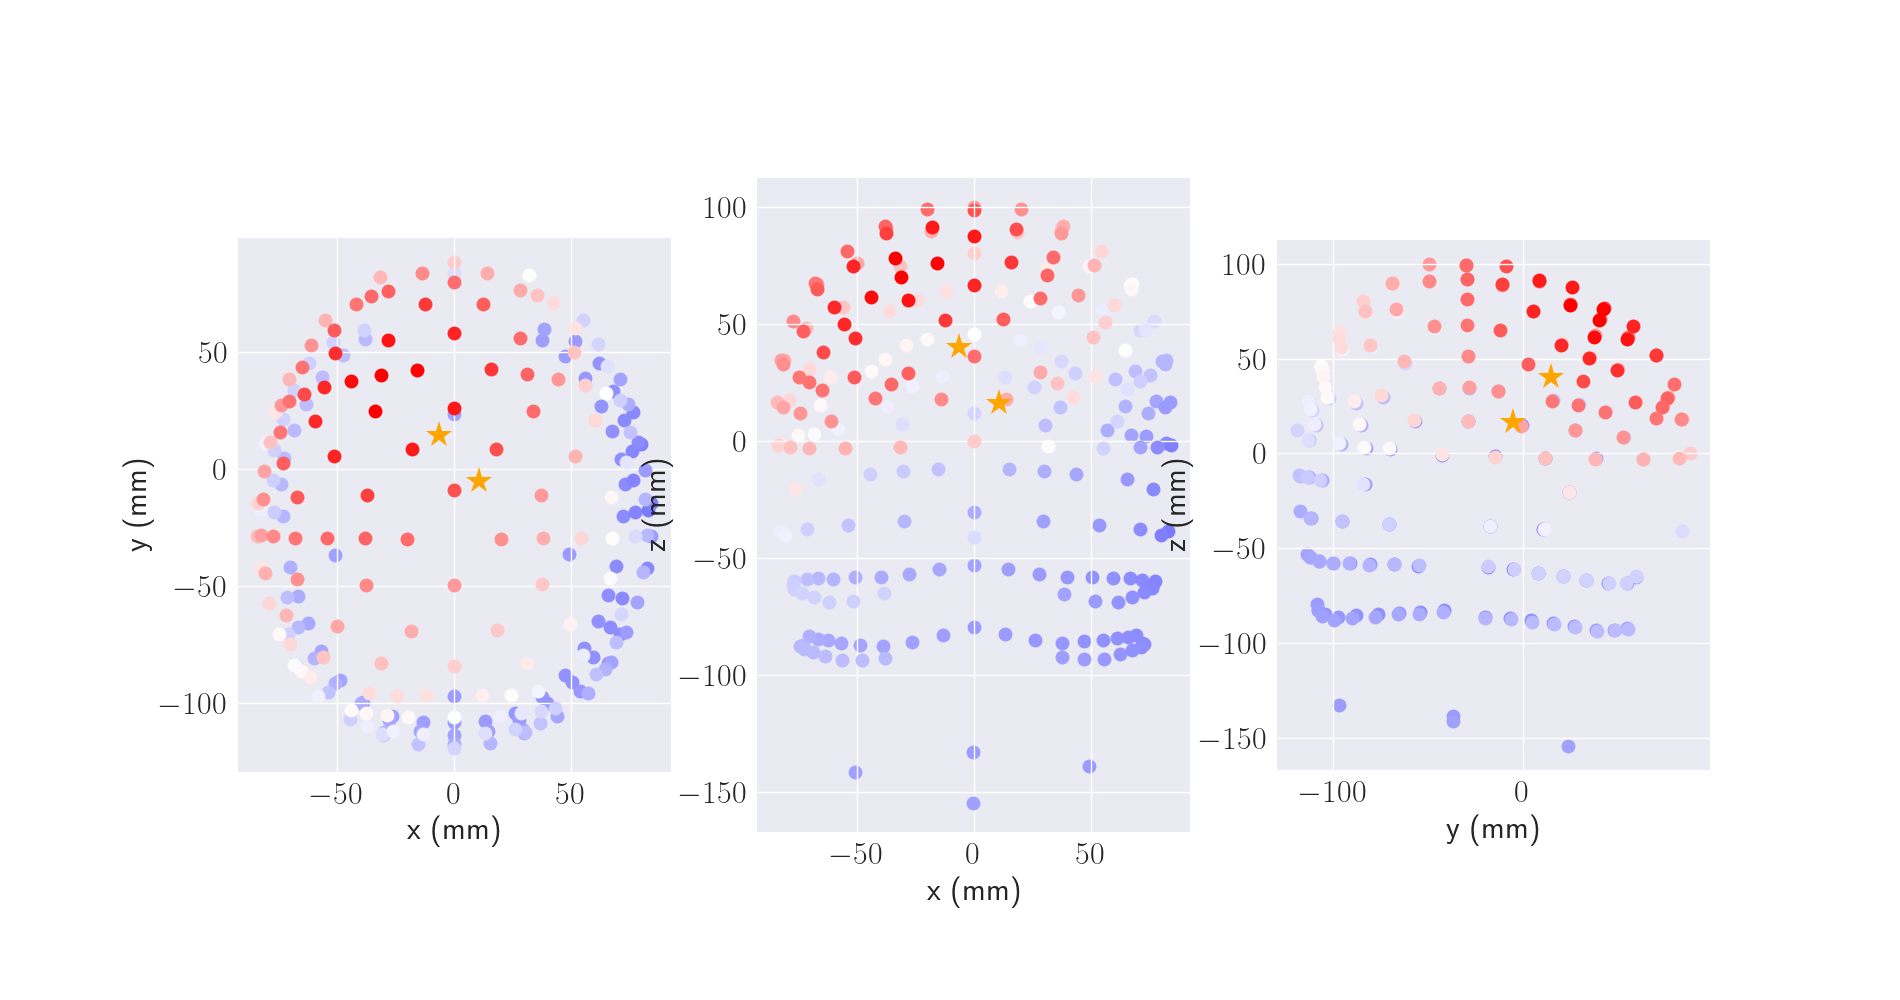
\includegraphics[width=\linewidth]{../Code/plots/finals/eeg_field_2_2.png}
    \caption{EEG for a sample containing two current dipole sources at random positions within the celebral cortex. The EEG measure is seen from both sides (x-, z-plane and y-, z-plane) and above (the x-, y-plane). EEG electrode locations are presented as filled circels, where the color of the fill represents the amplitude of the measured signal for the given electrode. The positions of the current dipole moments are marked with yellow stars.}
    \label{fig:dipole_area_result}
\end{figure}

\begin{figure}[!htb]
    \centering
    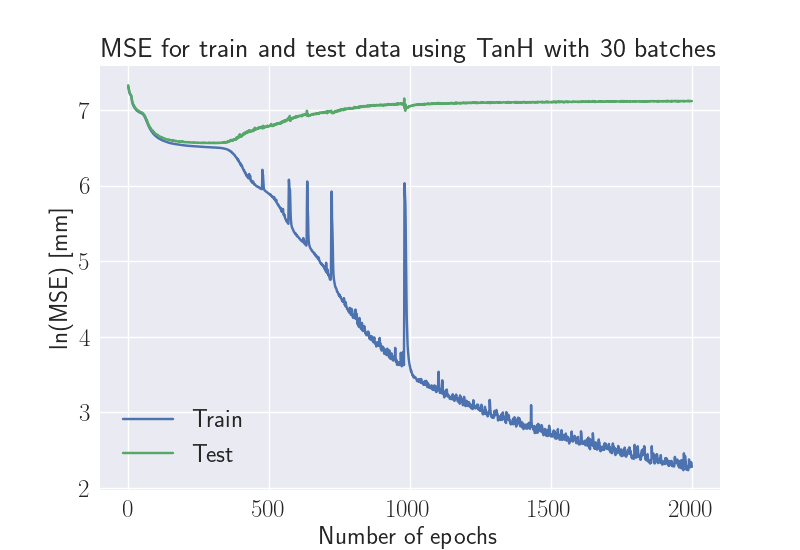
\includegraphics[width=\linewidth]{../Code/plots/finals/MSE_NN_2_10000_l1_TanH_30_2000.png}
    \caption{The validation accuracy for the simple Feed Forward Neural Network, predicting two current dipole sources.}
    \label{fig:dipole_area_result}
\end{figure}

\end{document}
